% Options for packages loaded elsewhere
\PassOptionsToPackage{unicode}{hyperref}
\PassOptionsToPackage{hyphens}{url}
\PassOptionsToPackage{dvipsnames,svgnames,x11names}{xcolor}
\documentclass[
  10pt,
  fontset=fandol]{ctexart}
\usepackage{xcolor}
\usepackage[margin=16mm]{geometry}
\usepackage{amsmath,amssymb}
\setcounter{secnumdepth}{-\maxdimen} % remove section numbering
\usepackage{iftex}
\ifPDFTeX
  \usepackage[T1]{fontenc}
  \usepackage[utf8]{inputenc}
  \usepackage{textcomp} % provide euro and other symbols
\else % if luatex or xetex
  \usepackage{unicode-math} % this also loads fontspec
  \defaultfontfeatures{Scale=MatchLowercase}
  \defaultfontfeatures[\rmfamily]{Ligatures=TeX,Scale=1}
\fi
\usepackage{lmodern}
\ifPDFTeX\else
  % xetex/luatex font selection
\fi
% Use upquote if available, for straight quotes in verbatim environments
\IfFileExists{upquote.sty}{\usepackage{upquote}}{}
\IfFileExists{microtype.sty}{% use microtype if available
  \usepackage[]{microtype}
  \UseMicrotypeSet[protrusion]{basicmath} % disable protrusion for tt fonts
}{}
\makeatletter
\@ifundefined{KOMAClassName}{% if non-KOMA class
  \IfFileExists{parskip.sty}{%
    \usepackage{parskip}
  }{% else
    \setlength{\parindent}{0pt}
    \setlength{\parskip}{6pt plus 2pt minus 1pt}}
}{% if KOMA class
  \KOMAoptions{parskip=half}}
\makeatother
\usepackage{longtable,booktabs,array}
\newcounter{none} % for unnumbered tables
\usepackage{calc} % for calculating minipage widths
% Correct order of tables after \paragraph or \subparagraph
\usepackage{etoolbox}
\makeatletter
\patchcmd\longtable{\par}{\if@noskipsec\mbox{}\fi\par}{}{}
\makeatother
% Allow footnotes in longtable head/foot
\IfFileExists{footnotehyper.sty}{\usepackage{footnotehyper}}{\usepackage{footnote}}
\makesavenoteenv{longtable}
\usepackage{graphicx}
\makeatletter
\newsavebox\pandoc@box
\newcommand*\pandocbounded[1]{% scales image to fit in text height/width
  \sbox\pandoc@box{#1}%
  \Gscale@div\@tempa{\textheight}{\dimexpr\ht\pandoc@box+\dp\pandoc@box\relax}%
  \Gscale@div\@tempb{\linewidth}{\wd\pandoc@box}%
  \ifdim\@tempb\p@<\@tempa\p@\let\@tempa\@tempb\fi% select the smaller of both
  \ifdim\@tempa\p@<\p@\scalebox{\@tempa}{\usebox\pandoc@box}%
  \else\usebox{\pandoc@box}%
  \fi%
}
% Set default figure placement to htbp
\def\fps@figure{htbp}
\makeatother
\setlength{\emergencystretch}{3em} % prevent overfull lines
\providecommand{\tightlist}{%
  \setlength{\itemsep}{0pt}\setlength{\parskip}{0pt}}
\usepackage{amsmath,amssymb,mathtools,needspace}
\xeCJKDeclareCharClass{CJK}{"2032,"0400->"04FF,"2160->"216B,"2460->"2473,"25A0,"25C7,"25CB,"25CF}
\IfFontExistsTF{Arial Unicode MS}{\xeCJKsetup{AutoFallBack=true}\setCJKfallbackfamilyfont{\CJKrmdefault}{Arial Unicode MS}}{}
\setcounter{secnumdepth}{0}
\setlength{\emergencystretch}{2em}
\allowdisplaybreaks
\usepackage{bookmark}
\IfFileExists{xurl.sty}{\usepackage{xurl}}{} % add URL line breaks if available
\urlstyle{same}
\hypersetup{
  pdftitle={单步法的收敛性和稳定性},
  colorlinks=true,
  linkcolor={Maroon},
  filecolor={Maroon},
  citecolor={Blue},
  urlcolor={Blue},
  pdfcreator={LaTeX via pandoc}}

\title{单步法的收敛性和稳定性}
\author{}
\date{}

\begin{document}
\maketitle

\subsection{5.4 单步法的收敛性和稳定性}\label{ux5355ux6b65ux6cd5ux7684ux6536ux655bux6027ux548cux7a33ux5b9aux6027}

\subsubsection{5.4.1 单步法的收敛性}\label{ux5355ux6b65ux6cd5ux7684ux6536ux655bux6027}

我们看到，数值解法的基本思想是，通过某种离散化手段，将微分方程转化为差分方程（代数方程）来求解。这种转化是否合理，还要看差分问题的解 \(y_n\) 当 \(h\to0\) 时是否会收敛到微分方程的准确解 \(y(x_n)\)。需要注意的是，如果只考虑 \(h\to0\)，那么节点 \(x_n=x_0+nh\) 对于固定的 \(n\) 将趋于 \(x_0\)，这时讨论收敛性是没有意义的。

\textbf{定义 5.2} 若一种数值方法对于任意固定的 \(x_n=x_0+nh\)，当 \(h\to0\)（同时 \(n\to\infty\)）时有 \(y_n\to y(x_n)\)，则称该方法是\textbf{收敛的}。

先就简单的初值问题

\[
\begin{cases}
y'=\lambda y,\\
y(0)=y_0
\end{cases}\tag{5.4.1}
\]

考察 Euler 方法的收敛性。方程 \(y'=\lambda y\) 的 Euler 格式是

\[
y_{n+1}=(1+\lambda h)y_n,\tag{5.4.2}
\]

它显然有解

\[
y_n=y_0(1+\lambda h)^n.
\]

由于这里 \(x_0=0,x_n=nh\)，有

\[
y_n=y_0\left[(1+\lambda h)^{\frac{1}{\lambda h}}\right]^{\lambda x_n}.
\]

再注意到当 \(h\to0\) 时，有

\[
(1+\lambda h)^{\frac{1}{\lambda h}}\to e,
\]

差分方程的解 \(y_n\) 当 \(h\to0\) 时确定收敛到原微分方程的准确解

\[
y(x_n)=y_0e^{\lambda x_n}.
\]

下面进一步考察一般的单步法。

所谓单步法，就是在计算 \(y_{n+1}\) 时只用到它前一步的信息 \(y_n\)。Taylor 级数法、

\href{../../source-images/pdf-134.jpeg}{原页}

Runge-Kutta 方法等都是单步法的例子。显式单步法的共同特征是，它们都是将 \(y_n\) 加上某种形式的增量得出 \(y_{n+1}\) 的，其计算公式形如

\[
y_{n+1}=y_n+h\varphi(x_n,y_n,h),\tag{5.4.3}
\]

其中 \(\varphi(x,y,h)\) 称为\textbf{增量函数}。

不同的单步法对应于不同的增量函数。不难就已知的几种单步法写出增量函数 \(\varphi(x,y,h)\) 的具体形式，譬如，对于 Euler 格式 (5.2.1)，有 \(\varphi=f(x,y)\)，而对于改进的 Euler 格式 (5.2.12)，有

\[
\varphi=\frac12[f(x,y)+f(x+h,y+hf(x,y))].\tag{5.4.4}
\]

关于单步法有下述收敛性定理。

\textbf{定理 5.1} 假设单步法 (5.4.3) 具有 \(p\) 阶精度，且增量函数 \(\varphi(x,y,h)\) 关于 \(y\) 满足 Lipschitz 条件

\[
|\varphi(x,y,h)-\varphi(x,\bar y,h)|\leqslant L_\varphi(y-\bar y),\tag{5.4.5}
\]

又设初值 \(y_0\) 是准确的，即 \(y_0=y(x_0)\)，则其\textbf{整体截断误差}

\[
y(x_n)-y_n=O(h^p).\tag{5.4.6}
\]

\textbf{证明} 设以 \(\bar y_{n+1}\) 表示取 \(y_n=y(x_n)\) 用格式 (5.4.3) 求得的结果，即

\[
\bar y_{n+1}=y(x_n)+h\varphi(x_n,y(x_n),h),\tag{5.4.7}
\]

其局部截断误差为 \(y(x_{n+1})-\bar y_{n+1}\)，由于所给方法具有 \(p\) 阶精度，按定义 5.1，存在定数 \(C\)，使

\[
|y(x_{n+1})-\bar y_{n+1}|\leqslant Ch^{p+1}.
\]

又由式 (5.4.7) 与式 (5.4.3)，得

\[
|\bar y_{n+1}-y_{n+1}|\leqslant|y(x_n)-y_n|+h|\varphi(x_n,y(x_n),h)-\varphi(x_n,y_n,h)|.
\]

利用假设条件 (5.4.5)，有

\[
|\bar y_{n+1}-y_{n+1}|\leqslant(1+hL_\varphi)|y(x_n)-y_n|,
\]

从而有

\[
\begin{aligned}
|y(x_{n+1})-y_{n+1}|&\leqslant|\bar y_{n+1}-y_{n+1}|+|y(x_{n+1})-\bar y_{n+1}|\\
&\leqslant(1+hL_\varphi)|y(x_n)-y_n|+Ch^{p+1},
\end{aligned}
\]

即对于整体截断误差 \(e_n=y(x_n)-y_n\) 成立下列递推关系式：

\[
|e_{n+1}|\leqslant(1+hL_\varphi)|e_n|+Ch^{p+1}.\tag{5.4.8}
\]

据此不等式反复递推，可得

\[
|e_n|\leqslant(1+hL_\varphi)^n|e_0|+\frac{Ch^q}{L_\varphi}[(1+hL_\varphi)^n-1].\tag{5.4.9}
\]

再注意到当 \(x_n-x_0=nh\leqslant T\) 时\footnote{对于任意实数 \(x\)，有 \(1+x\leqslant e^x\)，而当 \(x\geqslant-1\) 时，成立 \(0\leqslant(1+x)^n\leqslant e^{nx}\)。}

\begin{quote}
\textbf{校注（agent 补充，原书公式错误）}：式 (5.4.5) 原图右端为 \(L_\varphi(y-\bar y)\)，没有绝对值符号，已原样保留。标准 Lipschitz 条件及随后对非负误差的估计需要右端为 \(L_\varphi|y-\bar y|\)；当 \(y<\bar y\) 且 \(L_\varphi>0\) 时，原印右端为负，不能作为绝对差的上界。

\textbf{校注（agent 补充，原书指数错误）}：式 (5.4.9) 原印为 \(Ch^q/L_\varphi\)，已放大确认 \(q\) 并保留。按式 (5.4.8) 的等比求和，\(Ch^{p+1}\sum_{j=0}^{n-1}(1+hL_\varphi)^j=\dfrac{Ch^p}{L_\varphi}[(1+hL_\varphi)^n-1]\)，故此处指数应为 \(p\)；后页式 (5.4.10) 也用 \(p\)。
\end{quote}

\href{../../source-images/pdf-135.jpeg}{原页}

\[
(1+hL_\varphi)^n\leqslant(e^{nL_\varphi})^n\leqslant e^{hL_\varphi},
\]

最终得估计式

\[
|e_n|\leqslant|e_0|e^{TL_\varphi}+\frac{Ch^p}{L_\varphi}(e^{TL_\varphi}-1).\tag{5.4.10}
\]

由此可以断定，如果初值是准确的，即 \(e_0=0\)，则式 (5.4.6) 成立。证毕。

依据这一定理，判断单步法 (5.4.3) 的收敛性，归结为验证增量函数 \(\varphi\) 能否满足 Lipschitz 条件 (5.4.5)。

对 Euler 方法，由于其增量函数 \(\varphi\) 就是 \(f\)，故当 \(f\) 满足 Lipschitz 条件时它是收敛的。

再考察改进的 Euler 方法，其增量函数已由式 (5.4.4) 给出，这时有

\[
\begin{aligned}
&|\varphi(x,y,h)-\varphi(x,\bar y,h)|\\
&\leqslant\frac12\bigl[|f(x,y)-f(x,\bar y)|+|f(x+h,y+hf(x,y))\\
&\qquad-f(x+h,\bar y+hf(x,\bar y))|\bigr].
\end{aligned}
\]

假定 \(f\) 关于 \(y\) 满足 Lipschitz 条件，记 Lipschitz 常数为 \(L\)，则由上式推得

\[
|\varphi(x,y,h)-\varphi(x,\bar y,h)|\leqslant L\left(1+\frac{h}{2}L\right)|y-\bar y|.
\]

设限定 \(h\leqslant h_0\)（\(h_0\) 为定数），上式表明 \(\varphi\) 关于 \(y\) 的 Lipschitz 常数

\[
L_\varphi=L\left(1+\frac{h_0}{2}L\right),
\]

因此，改进的 Euler 方法也是收敛的。

类似地，不难验证其他 Runge-Kutta 方法的收敛性。

\subsubsection{5.4.2 单步法的稳定性}\label{ux5355ux6b65ux6cd5ux7684ux7a33ux5b9aux6027}

前面关于收敛性的讨论有个前提，必须假定数值方法本身的计算是准确的。实际情形并不是这样，差分方程的求解还会有计算误差，譬如由于数字舍入而引起的小扰动。这类小扰动在传播过程中会不会恶性增长，以致``淹没''了差分方程的``真解''呢？这就是差分方法的稳定性问题。在实际计算时，希望某一步产生的扰动值在后面的计算中能够被控制，甚至是逐步衰减的。

\textbf{定义 5.3} 若一种数值方法在节点值 \(y_n\) 上产生大小为 \(\delta\) 的扰动，在以后各节点值 \(y_m\)（\(m>n\)）上产生的偏差均不超过 \(\delta\)，则称该方法是\textbf{稳定的}。

稳定性问题比较复杂，为简化讨论，仅考察下列\textbf{模型方程} \(y'=\lambda y\)。为保证微分方程本身的稳定性，假定 \(\lambda<0\)。

先研究 Euler 方法的稳定性。模型方程 \(y'=\lambda y\) 的 Euler 格式为

\[
y_{n+1}=(1+h\lambda)y_n.\tag{5.4.11}
\]

设在节点值 \(y_n\) 上有一扰动值 \(\varepsilon_n\)，它的传播使节点值 \(y_{n+1}\) 产生大小为 \(\varepsilon_{n+1}\) 的扰动值，

\begin{quote}
\textbf{校注（agent 补充，原书指数错误）}：页首原印为 \((1+hL_\varphi)^n\leqslant(e^{nL_\varphi})^n\leqslant e^{hL_\varphi}\)，放大确认后按原式保留。由前页 \(nh\leqslant T\) 及 \(1+u\leqslant e^u\)，所需估计应为 \((1+hL_\varphi)^n\leqslant(e^{hL_\varphi})^n=e^{nhL_\varphi}\leqslant e^{TL_\varphi}\)，与本页式 (5.4.10) 一致。
\end{quote}

\href{../../source-images/pdf-136.jpeg}{原页}

假设用 \(y_n^*=y_n+\varepsilon_n\) 按 Euler 格式得出 \(y_{n+1}^*=y_{n+1}+\varepsilon_{n+1}\) 的计算过程不再有新的误差，则扰动值满足

\[
\varepsilon_{n+1}=(1+h\lambda)\varepsilon_n.
\]

可见扰动值满足原来的差分方程 (5.4.11)。这样，如果差分方程的解是不增长的，即有

\[
|y_{n+1}|\leqslant|y_n|,
\]

则它就是稳定的。这一论断对于下面将要研究的其他方法同样适用。

显然，为要保证差分方程 (5.4.11) 的解是不增长的，只要选取 \(h\) 充分小，使

\[
|1+h\lambda|\leqslant1.\tag{5.4.12}
\]

这说明 Euler 方法是\textbf{条件稳定的}，其稳定性条件为 \(h\leqslant-2/\lambda\)。记 \(\tau=-1/\lambda\)，则稳定性条件 (5.4.12) 可表示为

\[
h\leqslant2\tau.\tag{5.4.13}
\]

若自变量 \(x\) 表示时间，则 \(\tau\) 是一个具有时间量纲的量，工程上习惯地称它为\textbf{时间常数}。时间常数 \(\tau\) 可用来刻画原方程的解 \(y(x)\) 的衰减速度。事实上，在时间 \(\tau\) 内，解 \(y=y(0)e^{\lambda x}\) 衰减到它的 \(e^{-1}\) 倍。因此，\(\tau\) 越小，解 \(y(x)\) 衰减得越快。

Euler 方法的稳定性条件 \(h\leqslant2\tau\) 表明，时间常数 \(\tau\) 越小，稳定性对步长 \(h\) 的限制越苛刻。

再考察后退的 Euler 方法。对于模型方程 \(y'=\lambda y\)，其后退的 Euler 格式为

\[
y_{n+1}=y_n+h\lambda y_{n+1},
\]

解出 \(y_{n+1}\)，有 \(y_{n+1}=\dfrac{1}{1-h\lambda}y_n\)。由于 \(\lambda<0\)，这时恒成立

\[
\left|\frac{1}{1-h\lambda}\right|\leqslant1,
\]

从而有 \(|y_{n+1}|\leqslant|y_n|\)，因而后退的 Euler 方法\textbf{恒稳定}（或称\textbf{无条件稳定}）。

\textbf{例 5.5} 考察初值问题

\[
\begin{cases}
y'=-100y,\\
y(0)=1,
\end{cases}
\]

其准确解 \(y=e^{-100x}\) 是一个按指数曲线衰减得很快的函数，如图 5.4 所示。

对于所给方程 \(y'=-100y\)，其时间常数 \(\tau=0.01\)，因此，按式 (5.4.13)，为保证 Euler 方法稳定，步长 \(h\) 应使 \(\tau\) 不超过 \(2\tau=0.02\)。若取步长 \(h=0.025\)，则 Euler 格式的具体形式为

\[
y_{n+1}=-1.5y_n,
\]

计算结果列于表 5.5 的第二列。可以看到，Euler 方法的解 \(y_n\)（图 5.4 中用符号``■''标出）

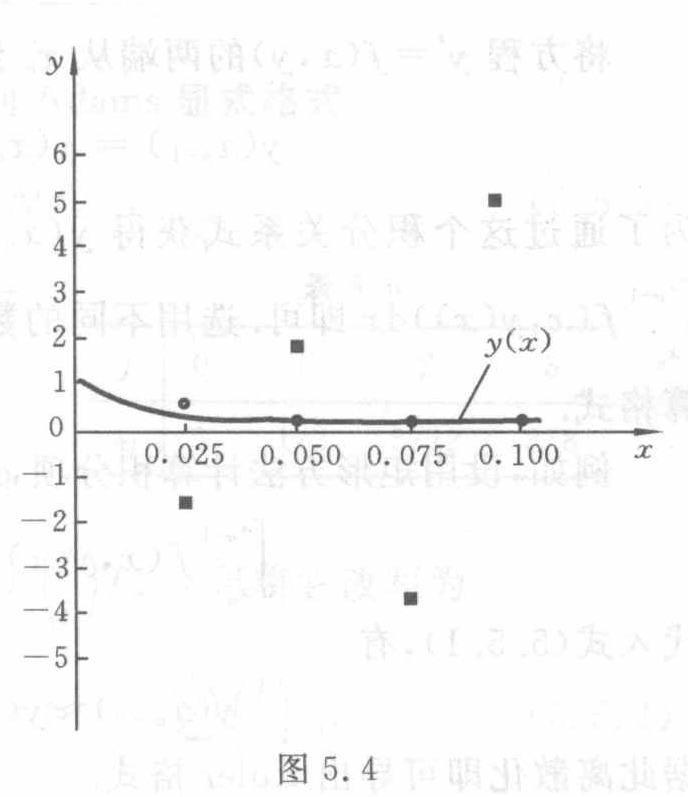
\includegraphics[width=0.85\linewidth,height=\textheight,keepaspectratio,alt={图 5.4 原图}]{../assets/ch05a/fig-5.4.png}

图 5.4（原图）：坐标系中画出衰减曲线 \(y(x)\)、正负交替且幅度增大的方形离散点，以及靠近横轴的圆形离散点。原图全部文字与刻度标签：\(x,y,y(x)\)；横轴 \(0.025,0.050,0.075,0.100\)；纵轴 \(-5,\allowbreak -4,\allowbreak -3,\allowbreak -2,\allowbreak -1,\allowbreak 0,\allowbreak 1,\allowbreak 2,\allowbreak 3,\allowbreak 4,\allowbreak 5,\allowbreak 6\)。点的说明随例 5.5 跨页续述。

\begin{quote}
\textbf{校注（agent 补充，原书文字/符号错误）}：例 5.5 原印``步长 \(h\) 应使 \(\tau\) 不超过 \(2\tau=0.02\)''，已经放大确认并保留。式 (5.4.13) 约束的是步长 \(h\)，应为``步长 \(h\) 应不超过 \(2\tau=0.02\)''；原句中的``使 \(\tau\)''使被约束量错置。
\end{quote}

\href{../../source-images/pdf-137.jpeg}{原页}

（接上页）在准确值 \(y(x_n)\) 的上下波动，计算过程明显地不稳定。

\textbf{表 5.5}

{\def\LTcaptype{none} % do not increment counter
\begin{longtable}[]{@{}lrr@{}}
\toprule\noalign{}
节点 & Euler 方法 & 后退的 Euler 方法 \\
\midrule\noalign{}
\endhead
\bottomrule\noalign{}
\endlastfoot
0.025 & −1.5 & 0.2857 \\
0.050 & 2.25 & 0.0816 \\
0.075 & −3.375 & 0.0233 \\
0.100 & 5.0625 & 0.0067 \\
\end{longtable}
}

再考察后退的 Euler 方法，取 \(h=0.025\) 时计算格式为

\[
y_{n+1}=\frac{1}{3.5}y_n.
\]

计算结果列于表 5.5 的第三列（图 5.4 中用符号``\(\bullet\)''标出），这时计算过程是稳定的。

\subsection{本节覆盖原页的校注记录}\label{ux672cux8282ux8986ux76d6ux539fux9875ux7684ux6821ux6ce8ux8bb0ux5f55}

下列记录按原页关联，含同页相邻小节的校注；计算时同时读取上文校注和完整原页。

\begin{itemize}
\tightlist
\item
  \texttt{ch05a-E004}：原书 PDF 页 134
\item
  \texttt{ch05a-E005}：原书 PDF 页 134
\item
  \texttt{ch05a-E006}：原书 PDF 页 135
\item
  \texttt{ch05a-E007}：原书 PDF 页 136
\end{itemize}

\end{document}
